%%%% Paramétrage du TD %%%%
\def\xxactivite{ \ifprof \normalsize{Application 1 -- Corrigé } \else  \ifcolle Colle \else Application 1\fi \fi} % \normalsize \vspace{-.4cm}
\def\xxauteur{\textsl{Xavier Pessoles}}


\def\xxnumchapitre{Chapitre 1 \vspace{.2cm}}
\def\xxchapitre{\hspace{.12cm} Approche énergétique}

\def\xxcompetences{%
\footnotesize{
\textsl{%
\textbf{Savoirs et compétences :}\\
\begin{itemize}[label=\ding{112},font=\color{ocre}] 
\item Mod2.C18.SF1 : Déterminer l’énergie cinétique d’un solide, ou d’un ensemble de solides, dans son mouvement par rapport à un autre solide.
\item Res1.C1.SF1 : Proposer une démarche permettant la détermination de la loi de mouvement.
%\item Mod1.C5.SF2 : Déterminer la puissance des actions mécaniques extérieures à un solide ou à un ensemble de solides, dans son mouvement rapport à un autre solide.
%\item Mod1.C5.SF3 : Déterminer la puissance des actions mécaniques intérieures à un ensemble de solides.
\end{itemize}}}}


\def\xxtitreexo{Micromanipulateur compact pour la chirurgie endoscopique ($\text{MC}^2\text{E}$)}
\def\xxsourceexo{\hspace{.2cm} \footnotesize{Concours Commun Mines Ponts 2016}}

\def\xxfigures{
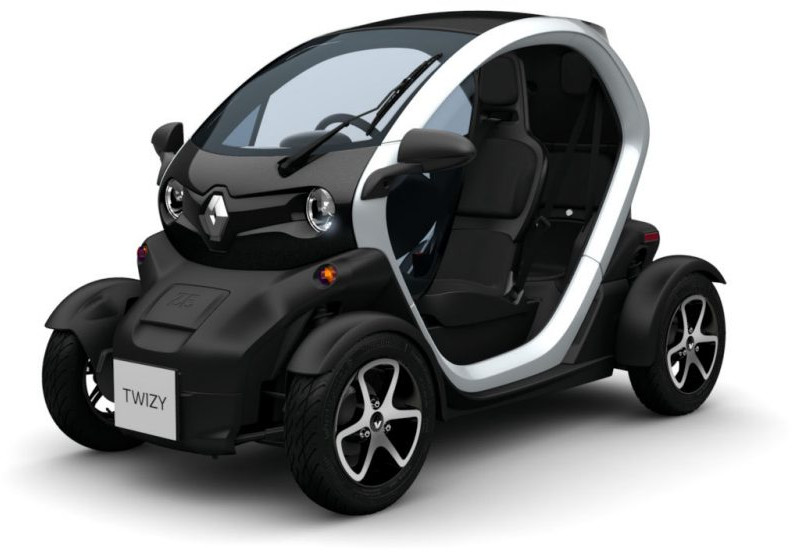
\includegraphics[width=.55\textwidth]{fig_01}
}%figues de la page de garde

\input{\repRel/Style/pagegarde_TD}
\setcounter{numques}{0}

\setlength{\columnseprule}{.1pt}

\pagestyle{fancy}
\thispagestyle{plain}


\vspace{5.2cm}

\def\columnseprulecolor{\color{ocre}}
\setlength{\columnseprule}{0.4pt} 

%%%%%%%%%%%%%%%%%%%%%%%

\setcounter{exo}{0}


\ifprof
\else
\begin{multicols}{2}
\fi
\section*{Mise en situation}

\ifprof
\else
Le robot $\text{MC}^2\text{E}$ est utilisé par des chirurgiens en tant que troisième main lors de l'ablation de la vésicule biliaire. La cinématique du robot permet de garantir que le point d'insertion des outils chirurgicaux soit fixe dans le référentiel du patient. 

Le robot est constitué de 3 axes de rotations permettant de mettre en position une pince. La pince est animée d'un mouvement de translation permettant de tirer la vésicule pendant que le chirurgien la détache du foie. 

\begin{center}
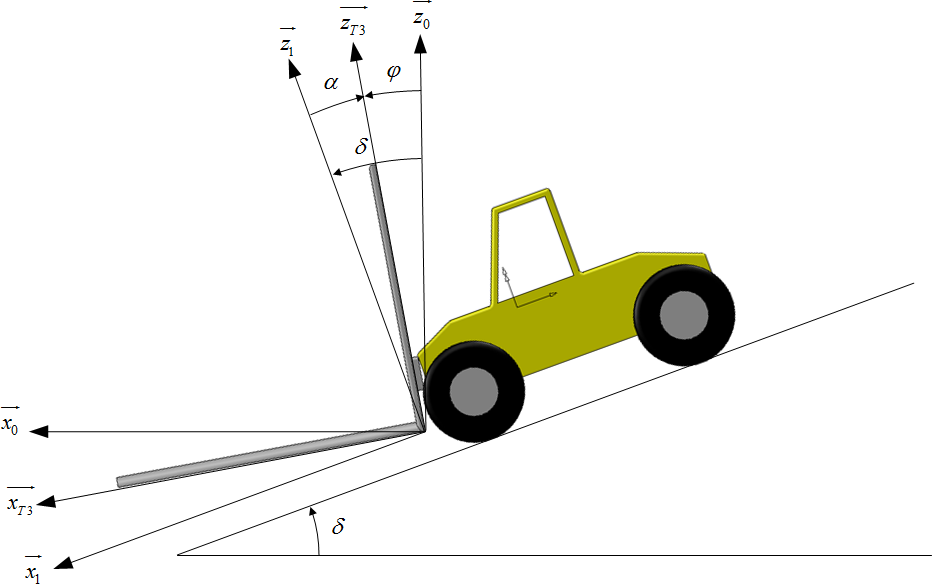
\includegraphics[width=\linewidth]{fig_02}
%\textit{}
\end{center}


Les blocs permettant de réaliser le mouvement de translation sont présentés ci-dessous.


\begin{center}
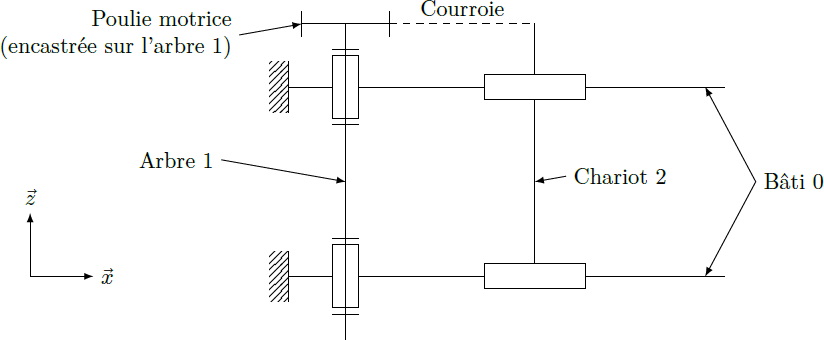
\includegraphics[width=\linewidth]{fig_05}
%\textit{}
\end{center}

Pour cela un moto réducteur entraîne via 3 systèmes poulie-courroie 3 galets qui entraînent la pince. 3 autres galets permettent de guider la pince. Au total 6 galets permettent d'entraîner et guider la pince par adhérence. Le premier étage de poulie-courroie permet de réduire la vitesse du moteur. Les deux autres étages ont un rapport de réduction unitaire (voir figure au verso). 
\fi



\begin{obj}
%Pour le montage d’essai, m
Modéliser l’équation de mouvement et la caractériser en fonction des actions mécaniques extérieures, du couple moteur et des grandeurs cinétiques appropriées.
\end{obj}

%La figure au verso donne un extrait du cahier des charges. 


%\begin{center}
%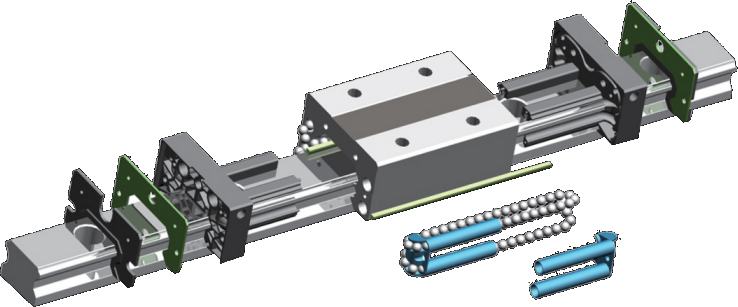
\includegraphics[width=\linewidth]{fig_03}
%%\textit{}
%\end{center}

\subsection*{Équation de mouvement}


%On rappelle que la transmission d’effort est représentée sur l’annexe 5. Un schéma cinématique simplifié minimal de cet axe pour cette étude est proposé en annexe 6. 
\ifprof
\else
\textbf{Hypothèses}
\begin{itemize}
\item La compensation de la pesanteur est parfaitement réalisée (système non étudié dans le cadre de cet exercice). On ne tiendra pas compte des actions mécaniques dues à la pesanteur par la suite.
\item Les axes de rotation du $\text{MC}^2\text{E}$ sont asservis en position. En conséquence, les repères liés aux solides \textbf{(1)}, \textbf{(2)} et \textbf{(3)} seront supposés fixes par rapport au repère lié au bâti \textbf{(0)} dont le repère associé est supposé galiléen.
\item L’instrument chirurgical est vertical.
\item Toutes les courroies sont inextensibles et il n’y a pas de glissement entre les galets et les courroies.
\item Tous les galets $G_i$ ont même rayon noté $\mathcal{R}_g$ et roulent sans glisser sur la pince \textbf{(4)} au niveau des points $I_1$ à $I_6$.
\item La poulie réceptrice est liée à un pignon. Ce pignon entraîne un deuxième pignon de même rayon primitif pour assurer la transmission de puissance. Il n’y a pas de glissement en leur point de contact.
\end{itemize}

Remarque : Dans la suite, toutes les vitesses sont définies par rapport au bâti \textbf{(0)}.

\textbf{Modélisation simplifiée du problème}
\begin{itemize}
\item La vitesse de rotation du rotor moteur M4 par rapport à son stator fixe (lié au bâti \textbf{(0)}) est notée $\omega_m(t)\vect{x_0}$  où $\omega_m(t)=\dfrac{\dd \theta_m(t)}{\dd t}$  (vitesse de rotation avant réduction de rapport $r$).
\item La poulie motrice a un rayon $R_i$ et tourne à la vitesse $\omega_i(t)$ (vitesse de rotation après réduction de rapport $r$).
\item La poulie réceptrice a un rayon $R_e$ et tourne à la vitesse $\omega_e(t)$.
\item Les deux pignons en contact ont même rayon primitif, supposé égal à $R_e$.
\item Le couple du stator sur le rotor moteur M4 est noté  $\vect{C_m}=C_m \vect{x_0}$.
\item L’action mécanique qu’exerce le ressort sur la pince (4) est modélisable par un glisseur noté 
$\torseurstat{T}{\text{ressort}}{4}=\torseurl{\vectf{\text{ressort}}{4}=-kz(t)\vect{z_0}}{\vect{0}}{O_4}$ où $O_4$ est le point de contact entre la pince \textbf{(4)} et le ressort, $k$ la raideur du ressort et $z(t)$ la variation de position de l’extrémité de \textbf{(4)} autour de la position d’équilibre.
\item On note $\vectv{O_4}{4}{0}=v(t)\vect{z_0}=\dfrac{\dd z(t)}{\dd t}\vect{z_0}$.
\item Les masses des courroies sont négligées.
\end{itemize}

\textbf{Données}
\begin{itemize}
\item $I_m$, moment d’inertie de l’arbre moteur par rapport à son axe de rotation.
\item $I_r$, moment d’inertie du réducteur par rapport à son axe de rotation de sortie.
\item $I_i$, moment d’inertie de la poulie, de rayon $R_i$, par rapport à son axe de rotation.
\item $I_e$, moment d’inertie de la poulie, de rayon $R_e$, par rapport à son axe de rotation.
\item $I_p$, moment d’inertie de chaque pignon, de rayon $R_e$, par rapport à son axe de rotation.
\item $I_g$, moment d’inertie de chaque galet $G_i$, de rayon $R_g$, par rapport à son axe de rotation.
\item $m_4$, masse de la pince \textbf{(4)}.
\item $r=\dfrac{\omega_i(t)}{\omega_m(t)}$, rapport de réduction constant du motoréducteur.
\end{itemize}

L’équation de mouvement est définie par l’équation différentielle suivante : $J\dfrac{\dd^2 \theta_m(t)}{\dd t^2}=C_m(t)-C_e(t)$  avec :
\begin{itemize}
\item $J$, inertie équivalente à l’ensemble en mouvement, ramenée sur l’arbre moteur ;
\item $C_e(t)$, couple regroupant l’ensemble des couples extérieurs ramenés à l’arbre moteur, notamment fonction de la raideur du ressort.
\end{itemize}

\fi


\subsection*{Travail demandé}


\question{Déterminer la relation entre $v(t)$ et $\omega_m(t)$. Sous hypothèse de conditions initiales nulles, en déduire la relation entre $z(t)$ et $\theta_m(t)$.}
\ifprof
\begin{corrige} ~\\
On a $\omega_i(t) = r\omega_m(t)$. De plus $\dfrac{\omega_e(t)}{\omega_i(t)}=\dfrac{R_i}{R_e} \Longleftrightarrow \omega_e(t)=\dfrac{R_i}{R_e}\omega_i(t)$ et donc :
$\omega_e(t)=\dfrac{R_i}{R_e}r\omega_m(t)$.

Enfin, $v(t)=R_g \omega_e(t) =R_g r \dfrac{R_i}{R_e}\omega_m(t)$. Les conditions initiales étant nulles, $z(t)=R_g r \dfrac{R_i}{R_e}\theta_m(t)$. 
\end{corrige}
\else
\fi


\question{Réaliser le graphe de structure associé à la translation de la pince.}
\ifprof
\begin{corrige} ~\\
\begin{center}
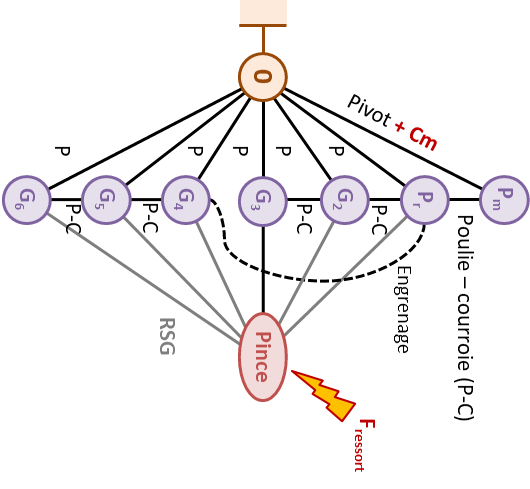
\includegraphics[width=.6\linewidth]{fig_07}
%\textit{}
\end{center}

\end{corrige}
\else
\fi

\question{Donner l’expression de l’énergie cinétique de l’ensemble en mouvement par rapport à \textbf{(0)}. Définir l’inertie équivalente $J$ ramenée sur l’axe du moteur M4 en fonction, notamment, des moments d’inertie, de $m_4$ et des données géométriques.}
\ifprof
\begin{corrige} ~\\

Tous les solides sont en mouvement << simples >> par rapport au référentiel galiléen. 
On a : 
$$
\mathcal{E}_c\left(E/\mathcal{R}_g\right) =
\dfrac{1}{2}I_m\omega_m(t)^2
+\dfrac{1}{2}\left(I_r+I_i\right)\omega_i(t)^2
+\dfrac{1}{2}\left(I_e+2I_p+6I_g\right)\omega_e(t)^2
+\dfrac{1}{2}m_4v(t)^2
$$
$$
\mathcal{E}_c\left(E/\mathcal{R}_g\right) =
\dfrac{1}{2}I_m\omega_m(t)^2
+\dfrac{1}{2}\left(I_r+I_i\right)\left( r\omega_m(t)\right)^2
+\dfrac{1}{2}\left(I_e+2I_p+6I_g\right)\left( \dfrac{R_i}{R_e}r\omega_m(t)\right)^2
+\dfrac{1}{2}m_4\left( R_g r \dfrac{R_i}{R_e}\omega_m(t) \right)^2
$$

$$
\mathcal{E}_c\left(E/\mathcal{R}_g\right) =
\dfrac{1}{2}\left(
I_m
+\left(I_r+I_i\right)r^2
+\left(I_e+2I_p+6I_g\right)\left( \dfrac{R_i}{R_e}r\right)^2
+m_4\left( R_g r \dfrac{R_i}{R_e} \right)^2\right)\omega_m(t)^2
$$

On a donc $J=I_m
+\left(I_r+I_i\right)r^2
+\left(I_e+2I_p+6I_g\right)\left( \dfrac{R_i}{R_e}r\right)^2
+m_4\left( R_g r \dfrac{R_i}{R_e} \right)^2$.
\end{corrige}
\else
\fi


\question{Effectuer un bilan des puissances extérieures et intérieures à ce même ensemble. Préciser l’expression analytique de chaque puissance.}
\ifprof
\begin{corrige} ~\\

On isole l'ensemble. 

\textbf{Bilan des puissances extérieures}
\begin{itemize}
\item Action du ressort : $\mathcal{P}\left(\text{ressort}\to 4/\mathcal{R}_g \right)=-kz(t)v(t)=-kz(t)R_g r \dfrac{R_i}{R_e}\omega_m(t)$.
\item Action du moteur : $\mathcal{P}\left(\text{moteur}\to 4/\mathcal{R}_g \right)=C_m\omega_m(t)$.
\item Action de la pesanteur : $\mathcal{P}\left(\text{pesanteur}\to E/\mathcal{R}_g \right)=0$ (La pesanteur est compensée par un système de compensation).
\end{itemize}

\textbf{Bilan des puissances intérieures}
Toutes les liaisons étant supposées parfaites, $\mathcal{P}_{\text{int}}\left(E\right)=0$.

\end{corrige}
\else
\fi


\question{Par l’application du théorème de l’énergie cinétique à l’ensemble en mouvement par rapport à \textbf{(0)}, déterminer l’expression du terme $C_e(t)$ en fonction des données du problème et de $\theta_m(t)$.}
\ifprof
\begin{corrige} ~\\
En appliquant le théorème de l'énergie cinétique on a : 
$
J\dot{\omega_m}(t)\omega_m(t) = -kz(t)R_g r \dfrac{R_i}{R_e}\omega_m(t)+C_m\omega_m(t) \Rightarrow 
J\dot{\omega}_m(t) = -k \left(R_g r \dfrac{R_i}{R_e}\right)^2\theta_m(t) +C_m.
$

En utilisant l'équation différentielle du mouvement on a alors : 
$C_e(t) = k \left(R_g r \dfrac{R_i}{R_e}\right)^2\theta_m(t)$.
\end{corrige}
\else
\fi

\ifprof
\else
\ifcolle
\else
\subsubsection*{Corrigé résumé}
\begin{enumerate}
\item $v(t)=R_g r \dfrac{R_i}{R_e}\omega_m(t)$ et $z(t)=R_g r \dfrac{R_i}{R_e}\theta_m(t)$. 
\item .
\item $J=I_m+\left(I_r+I_i\right)r^2 +\left(I_e+2I_p+6I_g\right)\left( \dfrac{R_i}{R_e}r\right)^2 +m_4\left( R_g r \dfrac{R_i}{R_e} \right)^2$.

\item $\mathcal{P}\left(\text{res}\to 4/\mathcal{R}_g \right)=-kz(t) \dfrac{R_g rR_i}{R_e}\omega_m(t)$, $\mathcal{P}\left(\text{mot}\to 4/\mathcal{R}_g \right)=C_m\omega_m(t)$, $\mathcal{P}\left(\text{pes}\to E/\mathcal{R}_g \right)=0$ et
$\mathcal{P}_{\text{int}}\left(E\right)=0$.
%\item $J\dot{\omega}_m(t) = -k \left(R_g r \dfrac{R_i}{R_e}\right)^2\theta_m(t) +C_m$.
\item $C_e(t) = k \left(R_g r \dfrac{R_i}{R_e}\right)^2\theta_m(t)$.
\end{enumerate}
\fi
\fi

\ifprof
\else
\end{multicols}
\fi

%\ifprof
%\else
%
%\vspace{1cm}
%\begin{center}
%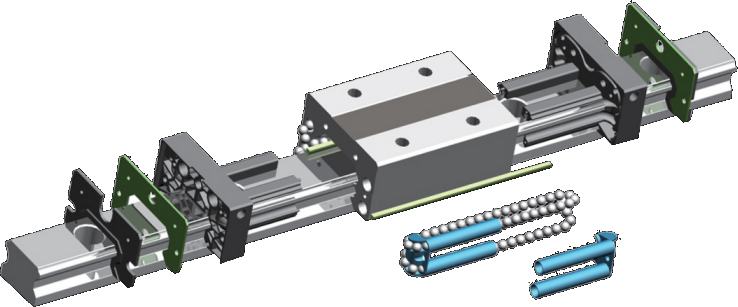
\includegraphics[width=\linewidth]{fig_03}
%%\textit{}
%\end{center}
%\fi
%\begin{center}
%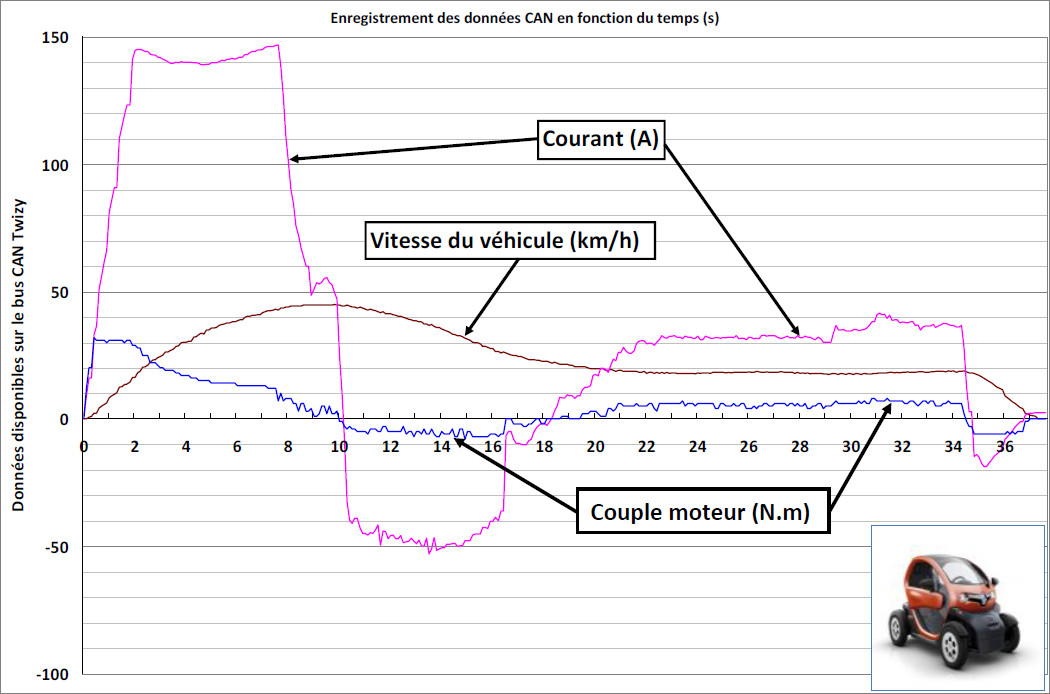
\includegraphics[width=\linewidth]{fig_04}
%%\textit{}
%\end{center}

\ifprof
\else
\begin{center}
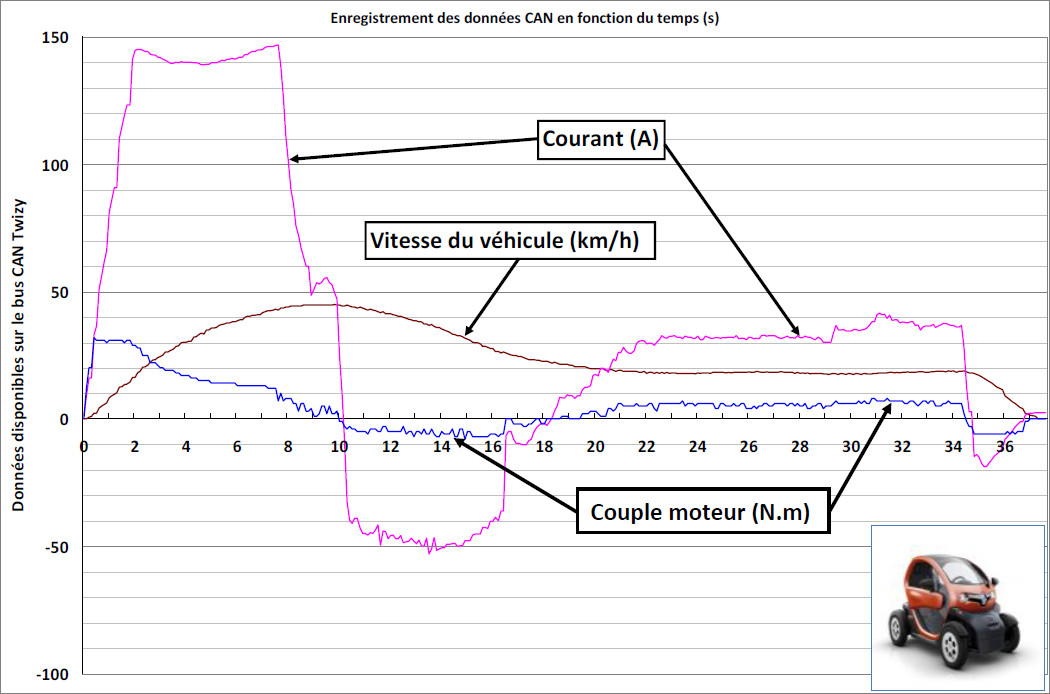
\includegraphics[width=\linewidth]{fig_04}
%\textit{}
\end{center}
\fi

